\chapter{Correlative Analysis and Visualization}

The chapter looks at some of the fundamentals of correlative analysis for dynamic systems, and discusses the merits and demerits of various correlative methods. We also look at historical techniques that have been used to visualize such data, and propose a visualization variant to capture changing correlation data over time.

\section{Correlation for Fault Analysis: Motivation}

In Chapter 2, we discussed some of the common methods for FDIR on complex systems, using linear system models that represent system state in terms of directly or indirectly telemetered values. However, there is key information that such an analysis can miss: the underlying connections between different telemetry channels. These connections can suggest semantic links, and even causations, between properties of the system, and can thus be used to link identified faults with unidentified changes of significance in other telemetered values. As such, a thorough study of the correlative attributes of a system can provide a framework with which its internal structure may be examined, and may even suggest modes of operation which can be used to understand higher-level system behavior.

\subsection{Covariance Matrices}

Covariance is defined as a measurement of the strength of correlation between two or more sets of random variables; i.e., it shows how much these variables ``change together." Statistically, for two variables $x$ and $y$, the covariance is the expected value of the product of the standard deviations of each of the variables:
\begin{equation} \label{eq:cov}
\mathrm{cov} = \text{E}[(x - \mu_{x})(y - \mu_{y})]
\end{equation}

Intuitively, it can be seen that a situation in which $x$ and $y$ both are much larger (or both much smaller) than their respective means results in a high covariance; a situation where $x$ is much larger than its mean, but $y$ is around its mean, will result in a small covariance. In this way, the correlation between these two variables is captured by a covariance measurement.

For a vector of random variables $\bar{x} \in \mathbb{R}^{n}$, there exists a symmetric covariance matrix $\Sigma \in \mathbb{R}^{n \times n}$ such that $\Sigma_{ij}$ is the covariance between $\bar{x}_{i}$ and $\bar{x}_{j}$. This matrix captures valuable correlative data about the system.

When looking at two sets of data, it can often be valuable to reduce their interdependence (i.e., how much they change in sync with each other) into a single number, or ``correlation coefficient." This coefficient is often a more generic version of the covariance, such that it can be used as straightforward metric to determine correlation between sets of times series data. It may even be used as input into visualization algorithms to affect shading or even positioning, as we will see in later chapters.

\subsection{Pearson Correlation Coefficient}

The Pearson Correlation Coefficient (PCC), also known as the Pearson Product-Moment Coefficient, is a metric of the linear relationship between two sets of data. It is essentially a scaled covariance, defined as \\
\begin{equation} \label{eq:pcc}
\text{PCC}_{X, Y} = \frac{\mathrm{cov}(X, Y)}{\sigma_{X} \sigma_{Y}}
\end{equation}

where $X$ and $Y$ are two vectors of data (or, in the case of the telemetry data sets we examine in this paper, times series of values over time for two telemetry channels). The PCC gives a quantified measurement of the linear correlation between the two vectors, in the form of a value in the range of $[-1, 1]$, where $1$ is a total positive correlation, $-1$ is a total negative correlation, and $0$ is no correlation at all.

The Pearson Correlation Coefficient carries with it a few important assumptions:

\begin{itemize}
\item Samples have values that are interval or ratio variables (not ordinal or categorical).
\item Sample pairs have a linear relationship (or, at least, these are the type of relationships you wish to see).
\item Sample pairs follow a bivariate normal distribution.
\end{itemize}

If the data doesn't fit the assumptions above, one of the two rank correlation coefficients discussed below may be more appropriate. In many of the spacecraft telemetry datasets we may encounter, the latter two assumptions will not hold, so the rank correlation coefficients will be of greater use.

\subsection{Spearman Rank Correlation Coefficient ($\rho$)}

The Spearman Rank Correlation Coefficient, or ``Spearman's Rho," is a type of correlation coefficient, which, like the PCC, seeks to quantify relationships between vectors of data, but which looks the ranking of variables within an ordering, rather than their linear relationship. This allows the coefficient to express relationship \textit{monotonicity}, in order to be less dependent on linearity of relationships. It actually makes uses of the PCC to do this, by calculating the PCC on the ranked data values.

Spearman's Rho is calculated by ranking the values for each variable, and then performing this calculation on those ranks:
\begin{equation} \label{eq:rho}
\rho_{X, Y} = 1 - \frac{6 \sum{d_{i}^{2}}}{n(n^{2}-1)},
\end{equation}

where $d_{i}$ is the difference in paired ranks, and $n$ is the number of observations. Like the PCC, Spearman's Rho takes the form of a value in the range of $[-1, 1]$, where $1$ is a total positive correlation, $-1$ is a total negative correlation, and $0$ is no correlation at all.

Spearman's Rho has assumptions which are far less restrictive than those of the PCC \cite{spearmans}:

\begin{itemize}
\item Samples have values that are interval, ratio or ordinal variables (not categorical).
\item Sample pairs must have a monotonic relationship (or, at least, these are the type of relationships you wish to see).
\end{itemize}

These relaxed assumptions allow for its confident application to a wider variety of real system data.

\subsection{Kendall Rank Correlation Coefficient ($\tau$)}

The Kendall Rank Correlation Coefficient, like ``Spearman's Rho," seeks to capture non-linear dependence by using the ordered ranks of the argument variables as input to the algorithm.

Kendall's Tau is defined as follows:
\begin{equation} \label{eq:tau}
\tau_{X, Y} = \frac{n_{c} - n_{d}}{n(n^{2}-1)/2},
\end{equation}

where $n_{c}$ is the number of ``concordant pairs" (pairs of variables with the same rank order across observations), $n_{d}$ is the number of ``discordant pairs" (pairs of variables with different rank order across observations), and $n$ is the number of observations.

Kendall's Tau carries with it the same assumptions as Spearman's Rho \cite{kendalls2}.

\section{Limitations of Traditional Correlative Techniques}

There are many limitations to the three traditional correlative techniques above, and it's important to understand them, even if the ultimate decision will be to use one of these techniques. Some of the major limitations are described below.

\subsection{Linearity Assumptions}

As discussed above, the PCC algorithm assumes that correlated data has a linear relationship between variables, and cannot adequately model nonlinear relationships. Many dynamic relationships that may be telemetered on a complex system are nonlinear, and will not be properly modeled using PCC. In contrast, the rank correlation methods model in terms of monotonicity, so they can capture many associative relationships that PCC cannot. Certain specially crafted pathological data sets can successfully confound PCC while being intuitively represented by rank correlation methods; see \cite{anscombe1973graphs} for the classic example of ``Anscombe's Quartet."

% \subsection{Multivariate Normal Distances vs. Elliptical Distances}

\subsection{Implied Causation}

One caveat of which a human operator must always be aware, especially when trying to build intuition and make conclusions based on correlative data, is that the formulations of correlation described above do not imply causation, and causation should not be inferred simply due to a high correlation score. However, correlation may \textit{suggest} causation, and can provide valuable next steps for data examination informed by expert knowledge.

\begin{figure}[h]
\centering
    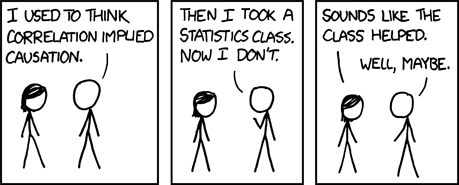
\includegraphics[width=0.5\columnwidth]{images/xkcd_correlation.png}
    \caption{A comical observation on the nature of correlation and causation. From \cite{xkcd_correlation}.}
    \label{fig:xkcd_correction}
\end{figure}


\subsection{Singular Value Decomposition and Principal Component Analysis}

We will briefly discuss the theory behind the Singular Value Decomposition and Principal Component Analysis, in order to use it as an analytical technique for correlative data later on in this thesis.

The Singular Value Decomposition, or SVD, is a way to diagonalize a given matrix in a pair of basis vectors \cite{kutz2013data}. If the matrix to be diagonalized is $A$, then the SVD may be written as
\begin{equation} \label{eq:svd}
A = \text{U} \Sigma \text{V}^{*},
\end{equation}

where \textbf{U} is a set of basis vectors expressing the range, $\Sigma$ is the diagonal matrix of singular values, and \textbf{V} is a set of basis vectors expressing the domain.

The SVD's two bases are orthonormal, and the SVD is guaranteed to exist for any matrix $A$, which cannot be said about the alternative diagonalization method of the eigenvalue decomposition \cite{kutz2013data}. The SVD allows us to project a matrix onto a low-dimensional representation in a formal way, a very useful quality for our spring system representations in this project.

Principal component analysis, or PCA, is a technique that makes heavy use of SVD. PCA takes an SVD of the covariance matrix of a series of observations in order to find the basis vectors and singular values that characterize the behavior. By looking at the magnitudes of the singular values, it becomes apparent which are significant, since the singular values are ordered and those of smaller magnitude can be elided in order to achieve a low-dimensional reduction to serve as a representation of the system \cite{kutz2013data}. This reduction consists of the ``principal components" of the system, and thus, PCA can be used to gain a fundamental understanding of how a system behaves, and how many principal modes it contains.

Note that it is important to normalize data before performing PCA, in order to avoid emphasizing data channels with large variances. Refer to \cite{shlens2014tutorial} for a detailed discussion of PCA.


\section{Visualization of Correlative Relationships}

As we discussed in the previous section, correlative relationships in a system can provide a useful view into the internal dynamics of state variables which a non-correlative approach could not. Because much of the motivation behind these variables is for discovery of new patterns and associations between variables, and as such, intuitive visualization to a human viewer is needed.

Correlative data is very high-dimensional; for a system with $n$ state variables, the correlative state looking back within a given time window is of size $\mathbb{R}^{n \times n}$. What's more, the correlative state changes over time as the time window slides across the state history, giving a total correlative state on the order of $\mathbb{R}^{n \times n \times t}$. For mission analysis over a 1,000-sample time window for an aerospace vehicle with 1,000 data channels, the correlative state has on the order of $10^{9}$ elements! Simultaneously visualizing this complex state in such a way that the data displayed to the user is maximized is a major challenge. Some of the difficulties of visualizing time series data, and the benefits of event identification and grouping, are studied in \cite{muller2003visualization}.

\subsection{Corrgrams}

A grid-based matrix representation of a matrix of correlative values, or ``corrgram," is a popular visualization used for correlation relationships in the research literature. In these visualizations, a state $\bar{x} \in \mathbb{R}^{n}$ is represented by a matrix $M \in \mathbb{R}^{n \times n}$, where $M_{ij}$ is shaded with a color hue to indicate the correlation score between $\bar{x}_{i}$ and $\bar{x}_{j}$.

\cite{yeh2007exploratory} suggests methods for visualizing correlations with schematic scatter plots and simple corrgrams. \cite{murdoch1996graphical} provides a method for more expressively visualizing correlative relationships between time series using embedded ellipse glyphs, but sacrifices dimensionality and screen space. Finally, a thorough survey of corrgram representations is given in \cite{friendly2002corrgrams}. 

For high-detail matrix structures that push the limits of on-screen display, \cite{yairi1992telemetry} shows a dense, 2D visualization of a subset of telemetry series data in which a measurement of ``association" is found through sorting, although the details of this correlative analysis are not given, and the applications were unclear to the authors as of the publication. Finally, \cite{cancro2007interactive} shows a colored, compact grid structure for maximizing telemetry display, although correlation is to be inferred by user inspection (i.e., noticing if two values happen to change similarly), rather than analyzed and displayed directly.

\subsubsection{Corrgram Limitations}

Corrgrams can only be used to display correlative state up to a certain level of dimensionality. After a certain point, the number of correlations which can be displayed on the screen is limited by screen space. The theoretical maximum, neglecting human perceptive elements, would be a correlation matrix where every pixel of a screen display is used to show a different pairwise correlation. If corrgram symmetry is exploited (i.e., if we only visualize the upper diagonal of the symmetric correlation matrix), we can reduce the number of visualized elements to $\frac{n^{2} - n}{2}$; however, on a generous modern screen resolution of 1920x1080, this reduces us to the capability of displaying correlations for only roughly 2,000 data channels. If we increase the pixel size to a much more reason 6x6 square for every data channel, we are reduced to roughly 300 displayable data channels. It is clear that screen space will be a major constraint, especially when precisely interaction with the data is necessary for detailed examination.

And it does seem that interaction will be a necessity. Even with a small number of data channels, horizontal and vertical labels to show data channel identifiers will not easily fit on the screen; therefore, an interaction system for showing the channel names for data pairs of interest is necessary. This interaction load slows down usage, though, and is likely to reduce utility of the visualization.

One final, major limitation of the corrgram visualization is that it only shows correlative state of the system at a single point in time; however, systems are dynamic, and their correlative states change as the systems transition between operational modes (including fault modes). If we are to see changes between modes, and to be able to identify these events as possible faults, we need a method to see correlative data change over time.

\subsubsection{Corrgram Example}

A monochrome corrgram comparison of the Pearson Correlation Coefficient, Spearman Rank Correlation Coefficient, and Kendall Rank Correlation Coefficient is shown in Fig.~\ref{fig:correlation_comparison}. Note that the strong negative linear correlation between data channels 4 and 5 is captured well by all three correlative measurement methods; however, the strong, nonlinear association between data channels 1 and 6 is not captured as strongly by the PCC due to its inability to model nonlinear relationships.

\begin{figure}[h]
\centering
    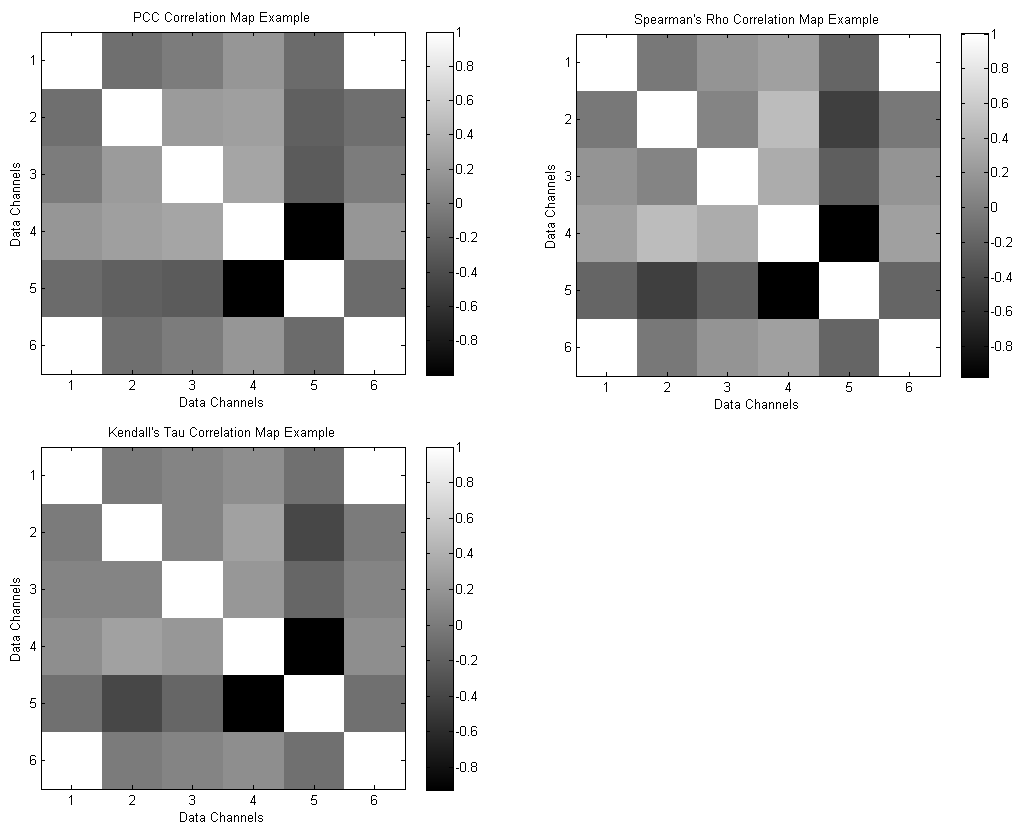
\includegraphics[width=\columnwidth]{images/correlation_comparison.png}
    \caption{Three common correlation coefficient algorithms are compared on a sample data set. Note that items 1 and 6 have a strong rank-based correlation, but the relationship is non-linear, resulting in a visibly lower correlation score within the PCC visualization. Also note the strong negative correlation between items 4 and 5.}
    \label{fig:correlation_comparison}
\end{figure}

\subsection{Animated Corrgrams}

Animated corrgrams are a potential solution to address the traditional corrgram's inability to capture changing correlative state over time. In an animated corrgram, the correlative state of a system is calculated over a retrospective time window, and every time new data is received, the correlative state is recalculated and redisplayed. This allows multiple ``views" of the current correlation during a run to be displayed, and facilitates the comparison of how correlation relationships change. We have been unable to find any examples of animated corrgrams used in previous research for displaying changing system state over time.

The next chapter will walk through the creation of an animated corrgram with real system data.

% \subsection{Alternatives to Correlation Score Techniques}

% \subsection{Applications of Correlation to Residual-Based Fault Analysis}

% Though we will be primarily examining the use of correlation for data discovery and root cause diagnosis, it's worth noting that correlation state data has been successfully used in previous research to create fault detection residuals to detect an understood fault state. In \cite{isermann1984process}, Isermann 

% Isermann paper

% Discussion of how this is using correlation between telemetry values to look for an understood fault state, rather than for data discovery (but it's still valuable!)

% \subsection{Distance Correlation}

% \subsection{Correlation Ratio}

% \subsection{Brownian Covariance}

% \subsection{Coefficient of Determination}

% \subsection{Polychloric Correlation}